%%%%%%%%%%%%%%%%%%%%%%%%%%%%%%%%%%%%%%%%%
% Beamer Presentation
% LaTeX Template
% Version 1.0 (10/11/12)
%
% This template has been downloaded from:
% http://www.LaTeXTemplates.com
%
% License:
% CC BY-NC-SA 3.0 (http://creativecommons.org/licenses/by-nc-sa/3.0/)
%
%%%%%%%%%%%%%%%%%%%%%%%%%%%%%%%%%%%%%%%%%

%----------------------------------------------------------------------------------------
%	PACKAGES AND THEMES
%----------------------------------------------------------------------------------------

\documentclass{beamer}

\mode<presentation> {



% The Beamer class comes with a number of default slide themes
% which change the colors and layouts of slides. Below this is a list
% of all the themes, uncomment each in turn to see what they look like.

%\usetheme{default}
\usetheme{AnnArbor}
%\usetheme{Antibes}
%\usetheme{Bergen}
%\usetheme{Berkeley}
%\usetheme{Berlin}
%\usetheme{Boadilla}
%\usetheme{CambridgeUS}
%\usetheme{Copenhagen}
%\usetheme{Darmstadt}
%\usetheme{Dresden}
%\usetheme{Frankfurt}
%\usetheme{Goettingen}
%\usetheme{Hannover}
%\usetheme{Ilmenau}
%\usetheme{JuanLesPins}
%\usetheme{Luebeck}
% \usetheme{Madrid}
%\usetheme{Malmoe}
%\usetheme{Marburg}
%\usetheme{Montpellier}
%\usetheme{PaloAlto}
%\usetheme{Pittsburgh}
%\usetheme{Rochester}
%\usetheme{Singapore}
%\usetheme{Szeged}
%\usetheme{Warsaw}

% As well as themes, the Beamer class has a number of color themes
% for any slide theme. Uncomment each of these in turn to see how it
% changes the colors of your current slide theme.

%\usecolortheme{albatross}
\usecolortheme{beaver}
%\usecolortheme{beetle}
%\usecolortheme{crane}
%\usecolortheme{dolphin}
%\usecolortheme{dove}
%\usecolortheme{fly}
%\usecolortheme{lily}
%\usecolortheme{orchid}
%\usecolortheme{rose}
%\usecolortheme{seagull}
%\usecolortheme{seahorse}
%\usecolortheme{whale}
%\usecolortheme{wolverine}

%\setbeamertemplate{footline} % To remove the footer line in all slides uncomment this line
%\setbeamertemplate{footline}[page number] % To replace the footer line in all slides with a simple slide count uncomment this line

%\setbeamertemplate{navigation symbols}{} % To remove the navigation symbols from the bottom of all slides uncomment this line
}

\usepackage{graphicx} % Allows including images
\usepackage{booktabs} % Allows the use of \toprule, \midrule and \bottomrule in tables
\usepackage{caption}
%----------------------------------------------------------------------------------------
%	TITLE PAGE
%----------------------------------------------------------------------------------------

\title[Photometric Redshifts]{Estimating the Photometric Redshifts of Galaxies Using Regression Techniques} % The short title appears at the bottom of every slide, the full title is only on the title page

\author[Momtaz, Salimi, Shakeri]{ A. Momtaz, M. H. Salimi, S.Shakeri}
%\rel{ Supervised by: P. Sahebsara, PhD.} % Your name
\institute[IUT] % Your institution as it will appear on the bottom of every slide, may be shorthand to save space
{
Department of Physics, Isfahan University of Technology, Isfahan 84156-8311, Iran. \\ % Your institution for the title page
\medskip
\textit{aidinmomtaz@ph.iut.ac.ir\\mhsalimi@ph.iut.ac.ir\\s.shakeri@iut.ac.ir} % Your email address
}
\date{July 7, 2021} % Date, can be changed to a custom date
\setbeamertemplate{caption}[numbered]
\begin{document}

\begin{frame}
\titlepage % Print the title page as the first slide
\end{frame}
%---------------------

%-----------------------

\begin{frame}
\frametitle{Overview} % Table of contents slide, comment this block out to remove it
\tableofcontents % Throughout your presentation, if you choose to use \section{} and \subsection{} commands, these will automatically be printed on this slide as an overview of your presentation
\end{frame}

%----------------------------------------------------------------------------------------
%	PRESENTATION SLIDES
%----------------------------------------------------------------------------------------
%----------------------------------------------------------------------------------------
%   Introduction
%----------------------------------------------------------------------------------------
\section{Introduction}
\subsection{Motivation}
\begin{frame}
    \begin{columns}[onlytextwidth]
    \begin{column}{.45\textwidth}
        \begin{figure}
            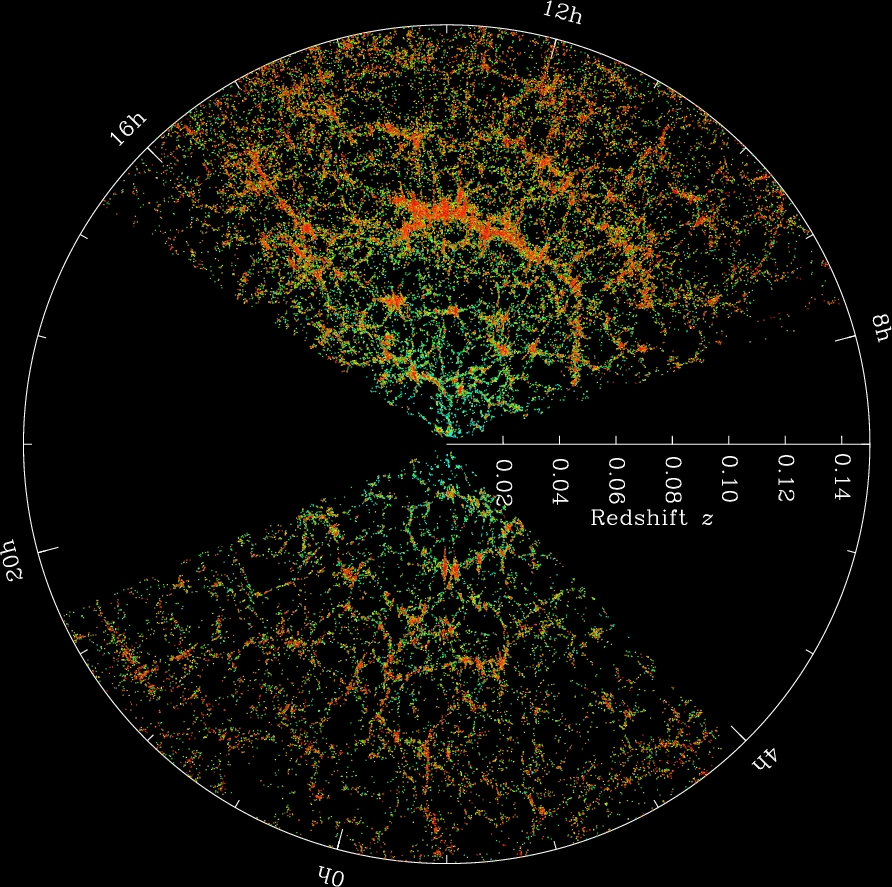
\includegraphics[width=\textwidth]{img/sdss_galaxy_map.jpg}
            \caption*{SDSS Galaxy Map}
        \end{figure}
    \end{column}
    \hfill
    \begin{column}{.45\textwidth}
    \begin{itemize}
        \item Possibility of Obtaining a Spectrum
        \item Sophisticated ML Algorithm
        \item Dark Energy and Dark Matter
    \end{itemize}
    \end{column}
    \end{columns}
    \end{frame}
\subsection{Spectroscopic and Photometric Redshifts}
\begin{frame}
    \begin{figure}
        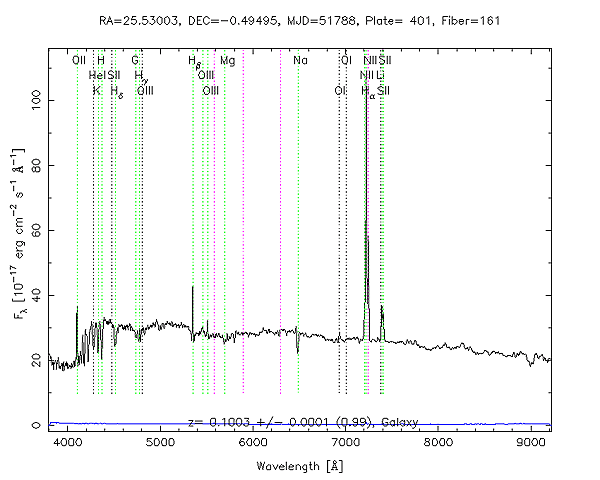
\includegraphics[scale=0.35]{img/galaxy_spectrum.png}
    \end{figure}
    \begin{equation}
        \lambda_{obs} = (1+z)\lambda_{em}
    \end{equation}
    \end{frame}
\begin{frame}
    \begin{figure}
        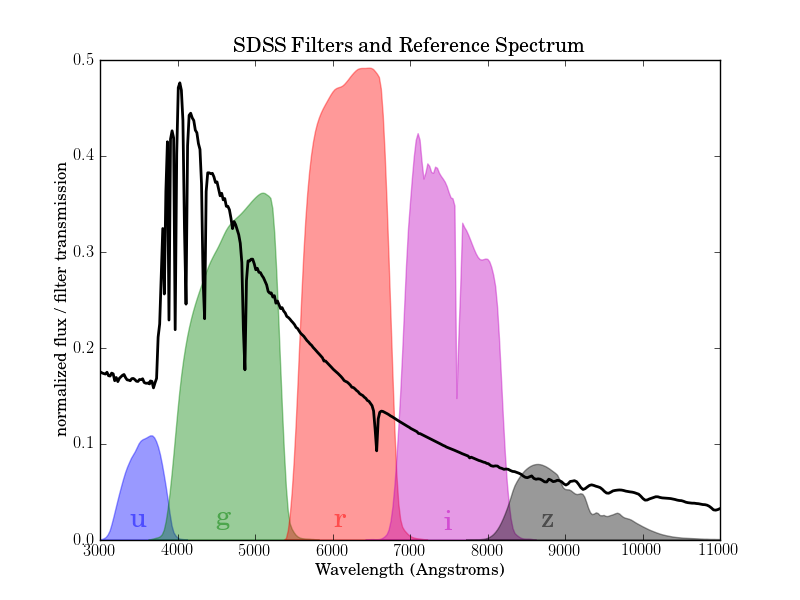
\includegraphics[scale=0.25]{img/sdss_plot.png}
    \end{figure}
    \begin{equation}
        u=m_{\text {ref }}-2.5 \log {10}\left[\int_{0}^{\infty} F(\lambda) S(\lambda) d \lambda\right]
    \end{equation}
    \end{frame}
\subsection{Machine Learning}
\begin{frame}
    \begin{description}
        \item[Decision Tree] \hfill \\ Decision trees map a set of input features to their corresponding output targets. This is done through a series of individual decisions where each decision represents a node (or branching) of the tree. 
        \\[0.2in]
        \pause
        \item[Random Forest] \hfill \\ Random forests are an ensemble learning method for classification, regression and other tasks that operates by constructing a multitude of decision trees at training time. 
    \end{description}
    % \begin{itemize}[<+->]
    %     \item Decision Tree
    %     \item Random Forest
    % \end{itemize}

    % \begin{block}{}
    %     \only<1>{Decision trees map a set of input features to their corresponding output targets. This is done through a series of individual decisions where each decision represents a node (or branching) of the tree.}
    %     \only<2>{Random forests are an ensemble learning method for classification, regression and other tasks that operates by constructing a multitude of decision trees at training time. }
    % \end{block} 
    \end{frame}


\begin{frame}
    \begin{figure}
        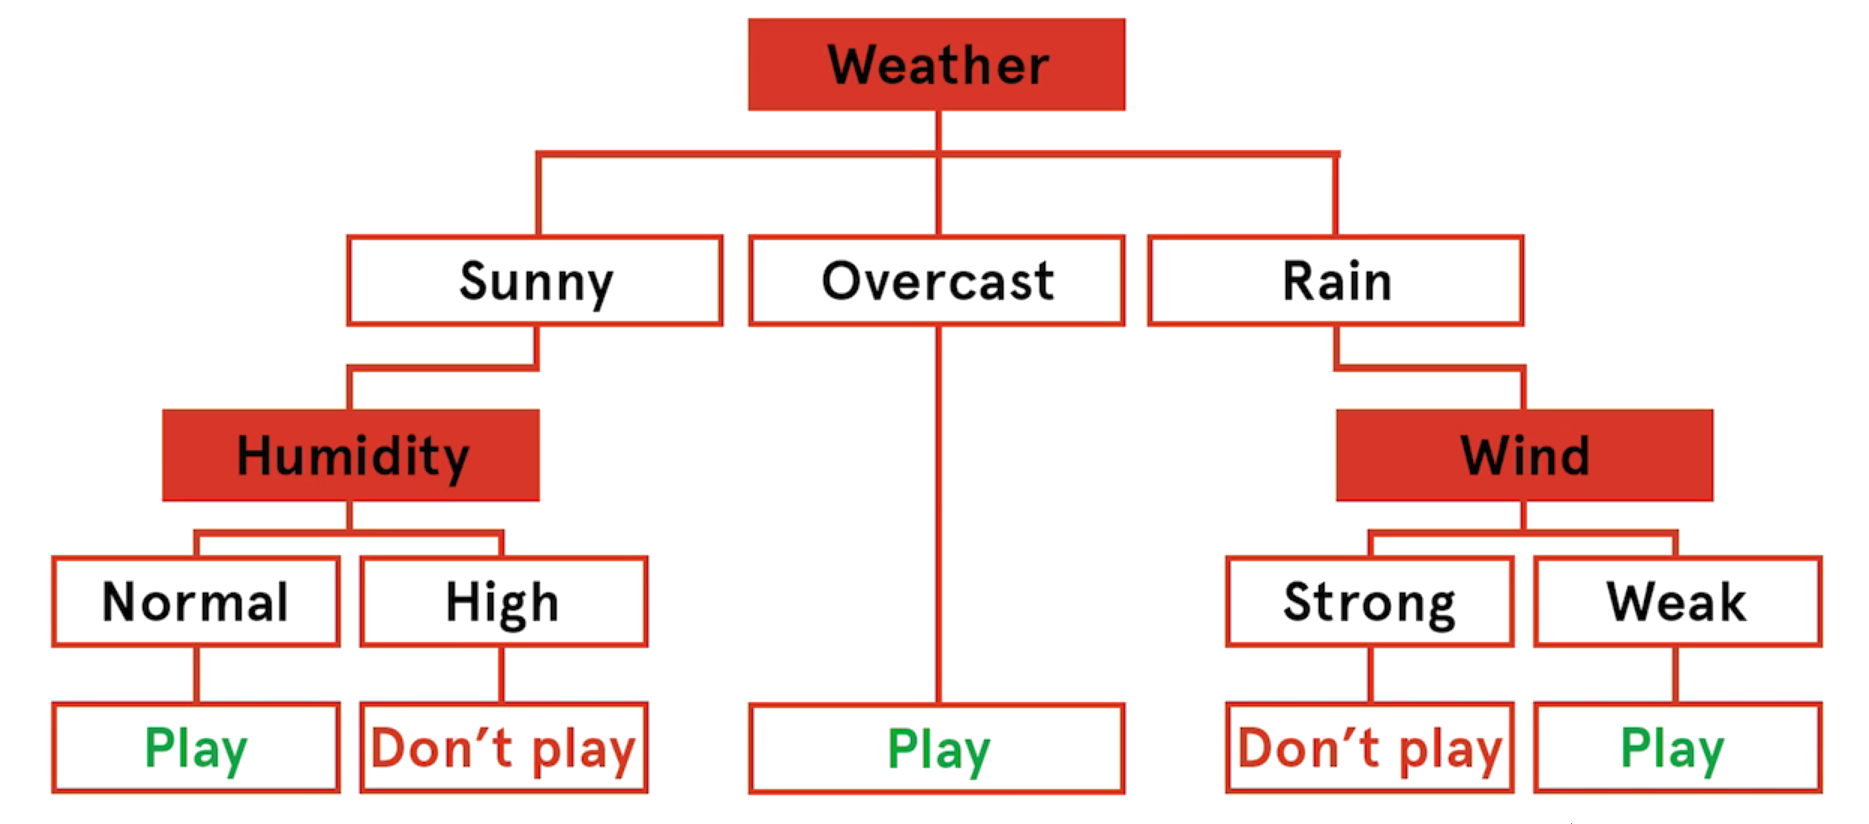
\includegraphics[scale=0.15]{img/decision_tree2.png}
        \caption{Schematic View of Decision Tree}
    \end{figure}
    \end{frame}

\begin{frame}
    \begin{figure}
        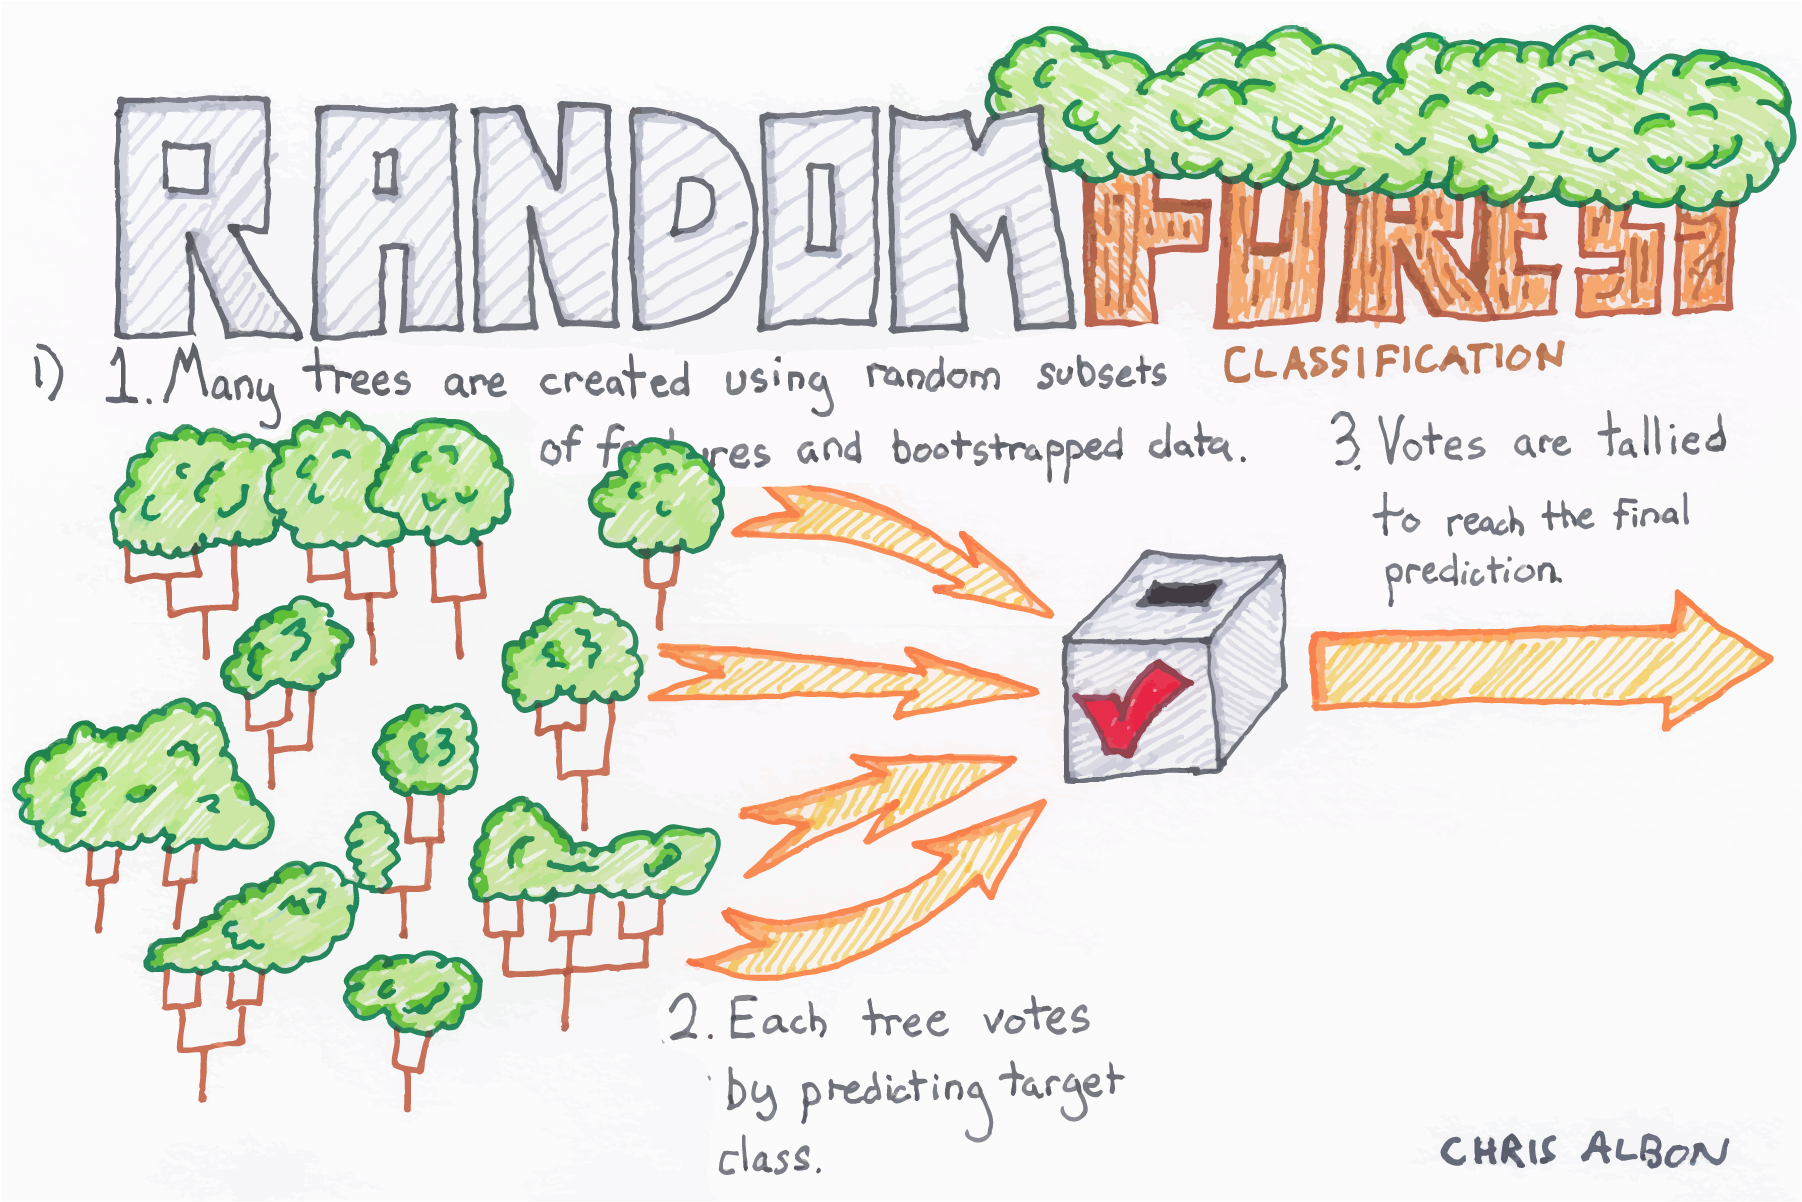
\includegraphics[scale=0.15]{img/Random_Forest.png}
        \caption{Schematic View of Random Forest}
    \end{figure}
    \end{frame}
%----------------------------------------------------------------------------------------
%   Methodology
%----------------------------------------------------------------------------------------
\section{Methodology}
\subsection{Data Preprocessing}
\subsection{Desicion Tree Algorithm}
\subsection{Random Forest Algorithm}
\subsection{Validation}
%----------------------------------------------------------------------------------------
%   Literature Survey
%----------------------------------------------------------------------------------------
\section{Literature Survey}
%----------------------------------------------------------------------------------------
%   Results & Disscusion
%----------------------------------------------------------------------------------------
\section{Results and Disscusion}


%----------------------------------------------------------------------------------------
\begin{frame}
\Huge{\centerline{Thanks For Your Attention :)}}
\end{frame}

%----------------------------------------------------------------------------------------
\end{document} 